\begin{table}[htdp]
\caption[Basic manipulations of the \asvd \ of an image]{Basic manipulations of the \asvd \ of an image matrix $\A{}$. The first transformation is the Hermitian conjugate $\A{*}$; besides a right-angle rotation it also involves a mirror flip. The pseudoinverse matrix $\Ap$ does not represent an image.}
\begin{center}
\begin{tabular}{ccc}
%
$\aesvd{*}$ &
$\aesvdt{*}$ &
$\apempp{*}$ \\
%
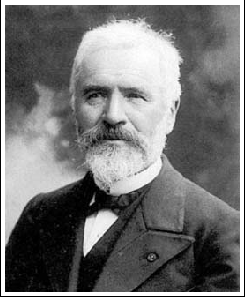
\includegraphics[ width = 1.22in ]{images/"information content I"/intro/default} &
\raisebox{0.2\height}{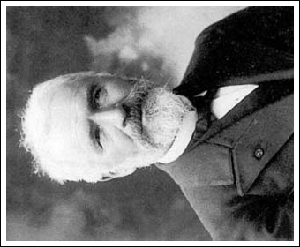
\includegraphics[ width = 1.5in ] {images/"information content I"/basics/transpose}} &
\raisebox{0.2\height}{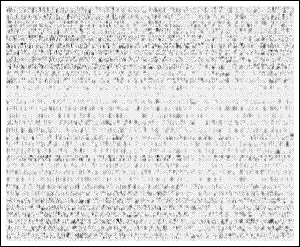
\includegraphics[ width = 1.5in ] {images/"information content I"/basics/mpp}} 
%
\end{tabular}
\end{center}
\label{tab:camille basics}
\end{table}

\endinput